\section{Mise en place du \textit{front-end}}

\begin{frame}{Mise en place du \textit{front-end}}
  \begin{block}{Les aspects du développement \textit{front-end}}
    \begin{itemize}
    \item La structure avec HTML.
    \item Le style avec CSS.
    \item Le comportement avec le Javascript.
    \end{itemize}
  \end{block}
\end{frame}

\subsection{HTML}
\begin{frame}{Structure HTML du projet}
  \begin{figure}
    \begin{center}
      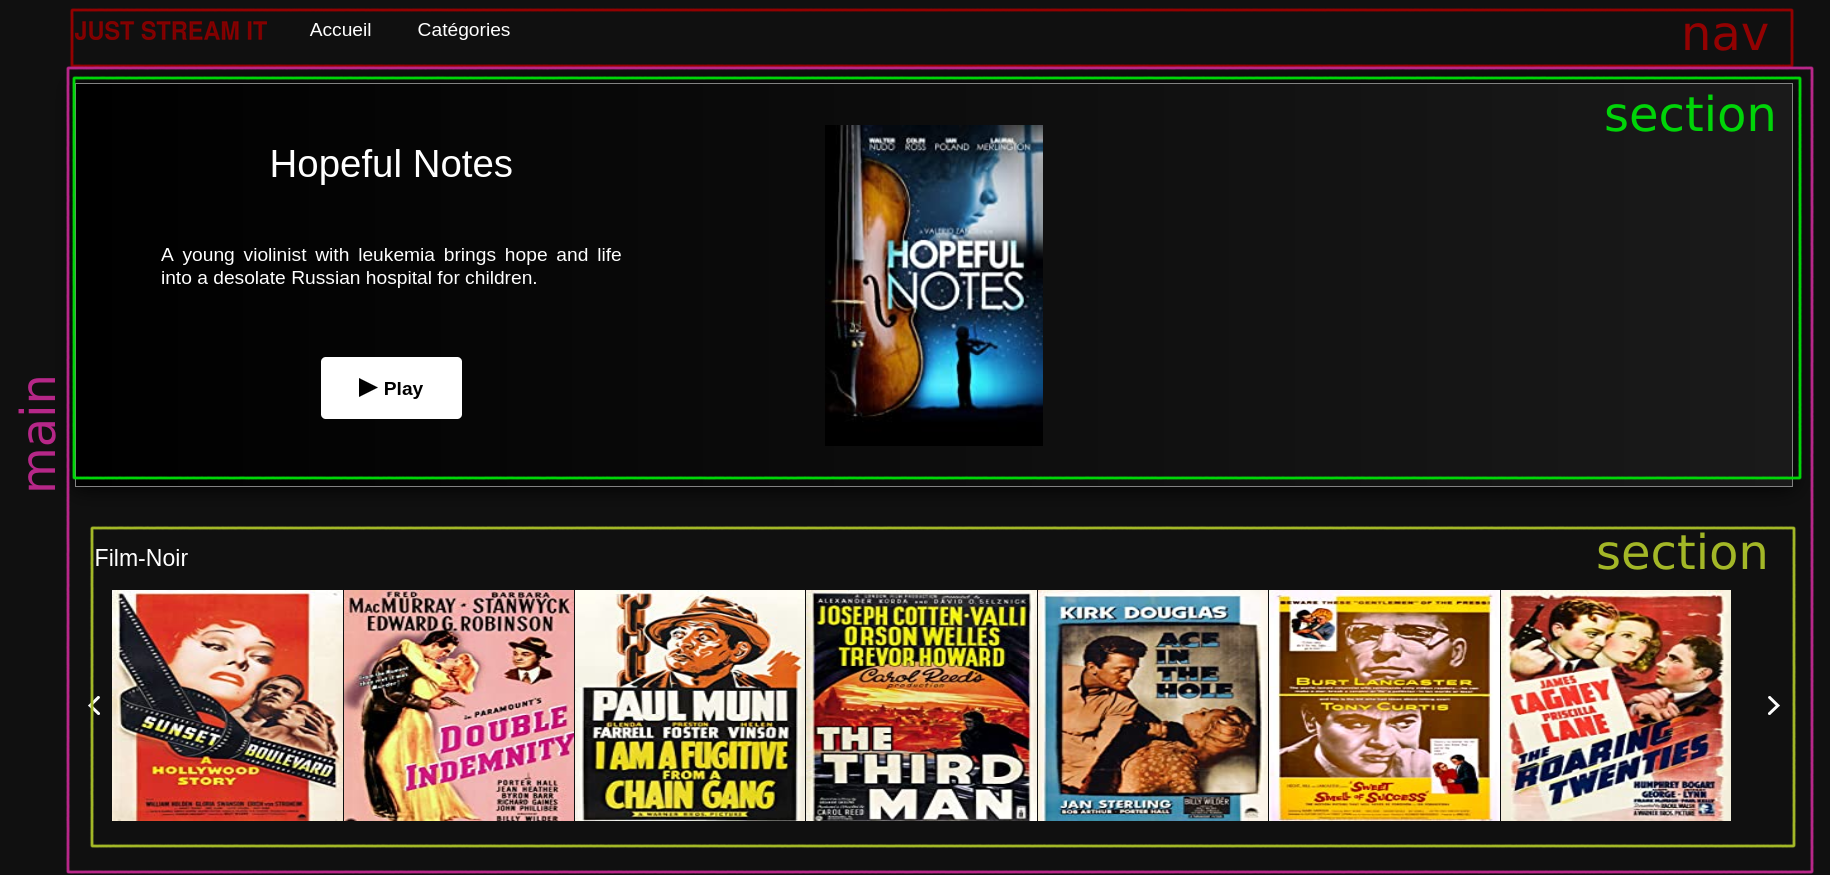
\includegraphics[scale=0.15]{img/html.png}
    \end{center}
    \caption{Éléments HTML de la page d'accueil}
  \end{figure}
\end{frame}

\subsection{CSS}

\begin{frame}[fragile]{Un CSS maintenable et \textit{scalable} avec SASS}  
  \begin{block}{Organisation}
    \begin{itemize}
    \item Séparation du style sur plusieurs fichiers
    \item Application du \textit{pattern} 7-1
    \end{itemize}
  \end{block}

  \begin{minted}{sass}
    @import 'base/reset';
    @import 'abstracts/mobile';
    @import 'themes/theme';
    @import 'layout/nav';
    @import 'pages/home';
    @import 'components/buttons';
    @import 'components/best_movie';                                                                                                                 @import 'components/category';
    @import 'components/movie_info';
  \end{minted}

\end{frame}

\begin{frame}[fragile]{Un CSS \textit{responsive}}
  \begin{block}{aze}
    \begin{itemize}
    \item Approche \textit{Mobile first} lors du développement.
    \item Utilisation d'une mixin SCSS pour gérer les \textit{media queries}.
    \end{itemize}
  \end{block}
  
  \begin{minted}[mathescape]{sass}
    @mixin for-mobile {
      @media screen and (max-width: 599px) {
        @content
      }
    }
  \end{minted}
\end{frame}

\begin{frame}[fragile]{Un CSS \textit{responsive}: exemple}
  
  \begin{minted}[mathescape]{sass}
    @include for-mobile {
      position: fixed;
      margin: 0;
      top: 0;
      left: 0;
      width: 100%;
      min-width: 0;
      height: 100%;
      max-height: 100%;
    }
  \end{minted}
\end{frame}

\begin{frame}[fragile]{Un CSS organisé avec la méthode BEM}
  % les autres méthodologie
  % pourquoi BEM ?
  % mise en place de BEM
  
  \begin{block}{La méthode BEM}
    \begin{itemize}
    \item Permet d'organiser le CSS.
    \item Extensible au SCSS.
    \item Signifie {\color{red}{\textit{Block}}} - {\color{violet}{\textit{Element}}} - {\color{teal}{\textit{Modifier}}}.
    \item Propose un formatage dans le choix des noms de classe CSS d'un projet.
    \end{itemize}    
  \end{block}

  \begin{block}{Un exemple de formatage}
    \textsc{\color{red}{nom\_bloc} \color{violet}{\_ \_ nom\_element} \color{teal}{- - nom\_modifier}}
  \end{block}
\end{frame}

\begin{frame}[fragile]{Le BEM appliqué au SASS}
  \begin{block}{En SASS}
    \scriptsize
    \begin{minted}{sass}
      .best_movie {
        &__title {
          &--blue {}
        }
      }
    \end{minted}
  \end{block}

  \begin{block}{En CSS}
    \scriptsize
    \begin{minted}{sass}
      .best_movie {}
      .best_movie best_movie__title {}
      .best_movie best_movie__title best_movie__title--blue {}
    \end{minted}
  \end{block}
\end{frame}

\subsection{Javascript}
\begin{frame}{Structure du code Javascript}
  \begin{block}{src/js}
    \begin{itemize}
    \item app.js
    \item movie.js
    \item carrousel.js
    \item category.js
    \item html.js
    \item api.js
    \end{itemize}
  \end{block}
\end{frame}

\begin{frame}{Utilisation de NPM}
  \begin{block}{Node Package Manager}
    \begin{itemize}
    \item N'est pas obligatoire pour le bon fonctionnement du projet.
    \item Permet de gérer les dépendances vers des bibliothèques javascript.
    \item Nous l'utilisons uniquement pour le test, le linter et autres
      outils indépendants du domaine métier.
    \end{itemize}
  \end{block}
\end{frame}

% \item app.js
% \item movie.js
% \item carrousel.js
% \item category.js
% \item html.js
% \item api.js

\begin{frame}[fragile]{Point d'entrée de l'application}
  \begin{block}{Fonctionnalité}
    \begin{itemize}
    \item Initialise les différentes catégories.
    \end{itemize}
  \end{block}
  
  \begin{minted}{javascript}
    async initAllCategories() {
      await Promise.all([	   
	this.initCategory('Biographies', 'Biography'),
	this.initCategory('Film-Noir', 'Film-Noir'),
	this.initCategory('Historique', 'History')
      ]);
    }
  \end{minted}  
\end{frame}

\begin{frame}[fragile]{Initialisation des catégories}
  \begin{minted}{javascript}
    async initCategory(name, genre) {
      let cat = new category.Category(name)

      const fetcher = new api.MovieFetcher();
      const movies = await fetcher.findByGenre(genre);

      for (let movie of movies) {
	cat.addMovie(movie);
      }

      this._categories.push(cat);	
    }
  \end{minted}
\end{frame}

\begin{frame}{Représentation des films}
  \begin{block}{Champs d'un objet \textit{Movie}}
    \tiny
    \begin{itemize}
    \item title
    \item image\_url
    \item genres
    \item release\_date
    \item rated
    \item imdb\_score
    \item directors
    \item actors
    \item duration
    \item countries
    \item box\_office		
    \item description
    \item long\_description
    \end{itemize}
  \end{block}
\end{frame}

\begin{frame}[fragile]{Représentation des catégories}
  \begin{block}{Constructeur de l'objet \textit{Category}}
    \begin{minted}{javascript}
      constructor(name) {
	this._name = name;
	this._movies = [];
	this._carrousel = new carrousel.Carrousel();
	this._root_element = null;
      }
    \end{minted}
  \end{block}
\end{frame}

\begin{frame}[fragile]{Mise en place du carrousel}

  \begin{block}{Représentation d'un carrousel}
    \begin{itemize}
    \item Utilisation de la classe \textit{Carrousel}.
    \item On peut ajouter un film au carrousel.
    \item On peut déplacer le carrousel vers la gauche ou la droite.
    \end{itemize}
  \end{block}
\end{frame}

\begin{frame}[fragile]{Animation du carrousel}

  \begin{block}{La classe \textit{CarrouselAnimation}}
    \small
    \begin{minted}{javascript}
      slide(speed=512, count=1) {
	const reference = this._list[0];
	let start = reference.offsetLeft;	
	html.animationLoop(function (dt) {
	    for(let movie of this._list) {
		html.moveElement(movie, speed * dt, 0);
	    }
	    
	    return Math.abs(reference.offsetLeft - start)
            < this._movie_width * count;
	}.bind(this));
      }
    \end{minted}
  \end{block}
\end{frame}

\begin{frame}[fragile]{Manipulation du code HTML}
  \begin{block}{Fonctionnalités de \textit{html.js}}
    \begin{minted}{javascript}
      export default {
        CategoryHTMLBuilder: CategoryHTMLBuilder,
        BestMovieHTMLBuilder: BestMovieHTMLBuilder,
        Modal: Modal,
        moveElement: moveElement,
        setElementPosition: setElementPosition,
        animationLoop: animationLoop
      };
    \end{minted}
  \end{block}
\end{frame}

\begin{frame}[fragile]{Génération du code HTML}
  \begin{block}{Fonctionnalités de \textit{html.js}}
    \begin{minted}{javascript}
      build(root_id) {
	let root = document.getElementById(root_id);
	let section = this.buildSection();
	root.appendChild(section);

	return section;
      }
    \end{minted}
  \end{block}
\end{frame}

\begin{frame}[fragile]{Génération du code HTML}
  \begin{block}{Fonctionnalités de \textit{html.js}}
    \small
    \begin{minted}{javascript}
      buildSection() {
	let section = document.createElement('section');
	section.classList.add('category');	
	let h2 = document.createElement('h2');
	h2.innerText = this._title;
	section.appendChild(h2);
	section.appendChild(this.buildCategoryContent());	
	return section;
      }
    \end{minted}
  \end{block}
\end{frame}

\begin{frame}[fragile]{Génération du code HTML}
  \begin{block}{Fonctionnalités de \textit{html.js}}
    \tiny
    \begin{minted}{javascript}
      buildCategoryContent() {
	let content = document.createElement('div');
	content.classList.add('category__content');

        let left_arrow = this.buildArrow('left');        
	left_arrow.addEventListener('click',this._left_callback);
	content.appendChild(left_arrow);
        
	let ul = document.createElement('ul');
        
	for (let movie of this._movies) {
	  ul.appendChild(this.buildMovie(movie));
	}

        // ...
    \end{minted}
  \end{block}
\end{frame}

\begin{frame}[fragile]{Récupération des informations \textit{via} l'API}
  \begin{block}{La classe \textit{MovieFetcher}}
    \begin{itemize}
    \item Permet de faire une recherche par genre, par ID ou par score IMDB. 
    \item Permet de créer un objet de type \textit{Movie} à partir
      d'un format JSON.
    \end{itemize}
  \end{block}

\end{frame}

\begin{frame}[fragile]{Recherche par genre}
  \tiny
  \begin{minted}{javascript}
    async findByGenre(name, count=7, url = null, results = []) {
      if (url === null) {
	url = `http://localhost:8000/api/v1/titles/?genre=${name}&sort_by=-imdb_score`;
      }
      
      const data = await fetch(url);
      const json_movie = await data.json();

      for (let result of json_movie.results) {
	const movie_result = await this.findByID(result.id);
	results.push(this.createMovieFromJSON(movie_result));
      }

      if (results.length < count) {
	await this.findByGenre(name, count, json_movie.next, results);
      }
      
      return results.slice(0, count);
    }
  \end{minted}
\end{frame}


\begin{frame}[fragile]{Création d'un objet \textit{Movie}}
  \small
  \begin{minted}{javascript}
    createMovieFromJSON(json_movie) {
      return new movie.Movie(json_movie.title,
      new URL(json_movie.image_url),
      json_movie.genres,
      new Date(json_movie.date_published),
      json_movie.rated,
      json_movie.imdb_score,
      json_movie.directors,
      json_movie.actors,
      json_movie.duration,
      json_movie.countries,
      json_movie.reviews_from_critics,			       
      json_movie.description,
      json_movie.long_description);
    }
  \end{minted}
\end{frame}

\begin{frame}{Gestion de la modale}
  \begin{block}{La classe \textit{Modal}}
    \begin{itemize}
    \item Permet d'afficher ou de cacher la fenêtre modale.
    \item Permet de mettre à jour les informations montrées.
    \end{itemize}
  \end{block}
\end{frame}

\begin{frame}[fragile]{HTML de la modale}
  \begin{block}{Entête de la modale}
    \tiny
    \begin{minted}{html}
      <div class="movie_info">
      <div class="movie_info__header">
      <span class="movie_info__header__title">Titre</span>
      <span class="movie_info__header__close">&times;</span>	  
      </div>
    \end{minted}
  \end{block}

  \begin{block}{Contenu de la modale}
    \tiny
    \begin{minted}{html}
      <div class="movie_info__content">
      <img src="https://via.placeholder.com/256" alt="image film"></img>

      <table>
      <tr>
      <th>Genres</th>
      <td id="movie_info__content__genres"><ul></ul></td>
      </tr>
      <tr>
      <th>Sortie</th>
      <td id="movie_info__content__release_date"></td>
      </tr>
      <!-- ... -->
    \end{minted}
  \end{block}

\end{frame}

\begin{frame}[fragile]{Visibilité de la modale}
  \begin{block}{Montrer}
    \tiny
    \begin{minted}{javascript}
      show(movie) {
        if (this._is_visible === false) {
	  this.update(movie);
	  this._is_visible = true;
	  this._root.style.display = 'inline-block';
        }
      }
    \end{minted}
  \end{block}

  \begin{block}{Cacher}
    \tiny
    \begin{minted}{javascript}
      hide() {
        if (this._is_visible === true) {
	  this._is_visible = false;
	  this._root.style.display = 'none';
        }
      }
    \end{minted}      
  \end{block}
\end{frame}

\begin{frame}[fragile]{Mise à jour de la modale}
  \begin{block}{Récupération des élements du DOM de la modale (extrait)}
    \tiny
    \begin{minted}{javascript}
      update(movie) {
        const prefix = '#movie_info__content__';
        
        const elements = {
          'title': document.querySelector('.movie_info__header__title'),
          'img': document.querySelector('.movie_info__content img'),
          'genres': document.querySelector(prefix + 'genres ul'),
          'release': document.querySelector(prefix + 'release_date'),
          'rated': document.querySelector(prefix + 'rated'),
          'imdb': document.querySelector(prefix + 'imdb'),
          'directors': document.querySelector(prefix + 'directors ul'),
          'actors': document.querySelector(prefix + 'actors ul'),
          'duration': document.querySelector(prefix + 'duration'),
          'countries': document.querySelector(prefix + 'countries ul'),
          'box-office': document.querySelector(prefix + 'box_office'),
          'summary': document.querySelector(prefix + 'summary')
        };

        // ...
    \end{minted}
  \end{block}
\end{frame}

\begin{frame}[fragile]{Mise à jour de la modale}
  \begin{block}{Modification du HTML (extrait)}
    \tiny
    \begin{minted}{javascript}
      elements['title'].innerText = movie.title;
      elements['img'].setAttribute('src', movie.image_url);
      
      this.buildList(elements['genres'], movie.genres);    
      elements['release'].innerText = movie.release_date.toDateString();
      elements['rated'].innerText = movie.rated;
      elements['imdb'].innerText = movie.imdb_score;
      this.buildList(elements['directors'], movie.directors);
      this.buildList(elements['actors'], movie.actors);

      // ...
    \end{minted}
  \end{block}
\end{frame}
